\chapter{进程模板}

进程模板定义了协议进程的属性、方法和通信手段,在使用sbid进行协议建模时,进程模板是必不可少的部分。

\section{自定义类型}
在[协议>概览]下,点击小工具栏上的[自定义类型]按钮,即可创建新的自定义类型的类图,如图\ref{create_usertype}所示。
    \begin{figure}[h]
	\centering
	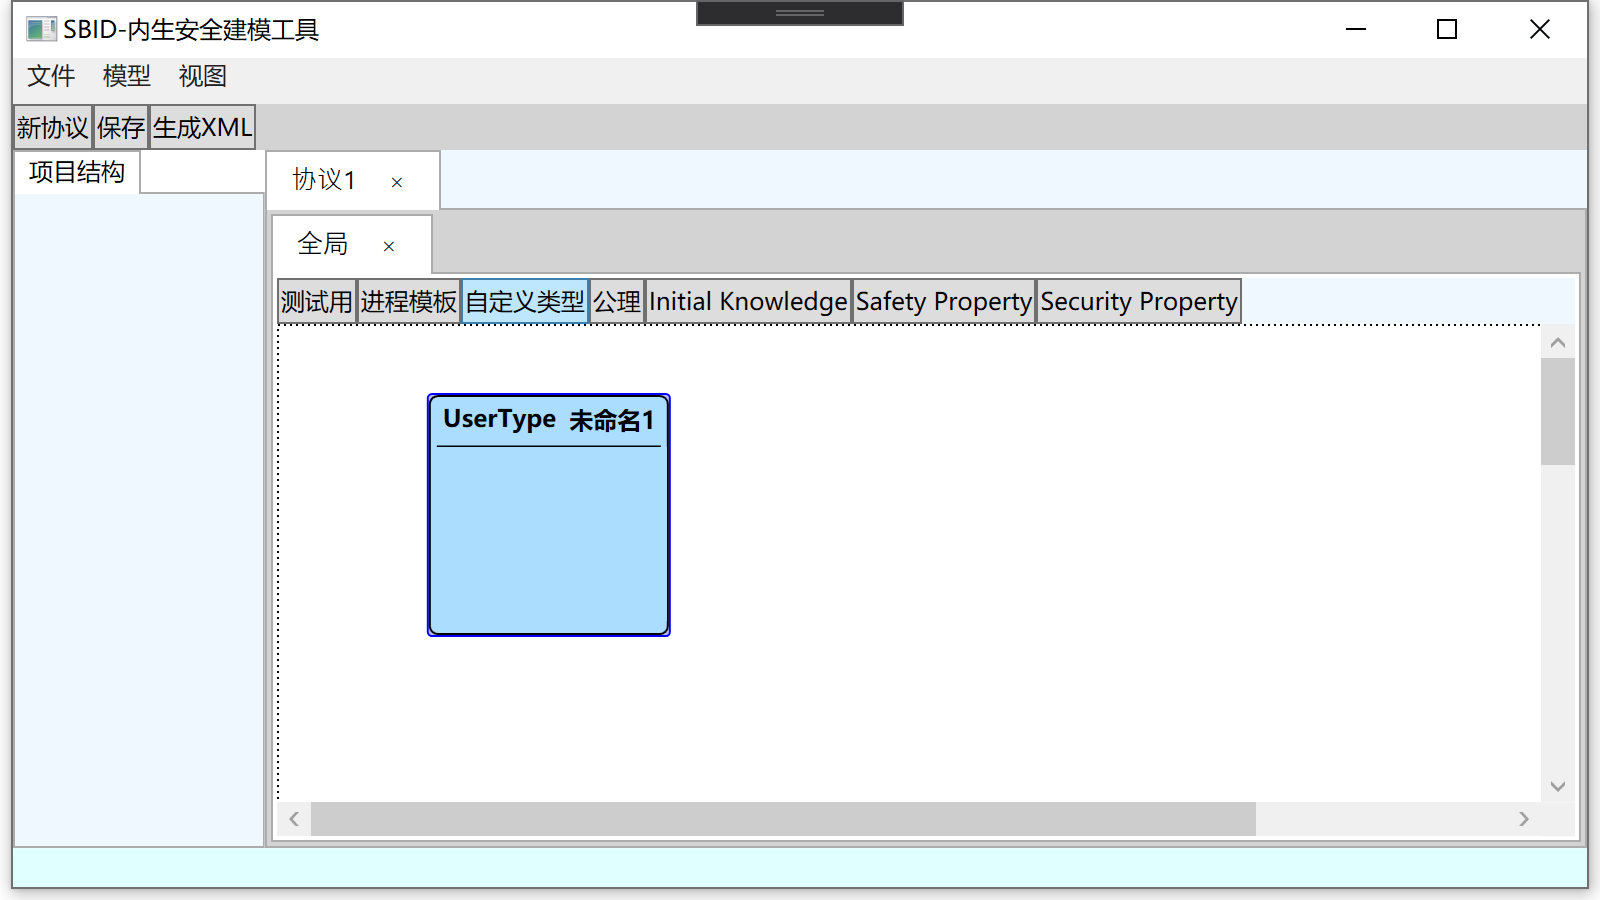
\includegraphics[width=12cm,height=6.75cm]{imgs/create_usertype.png}
	\caption{新创建的自定义类型}
	\label{create_usertype}
	\end{figure}
\par
在sbid工具中,默认为用户内置了$int$和$bool$两种基本数据类型,用户可以使用它们定制更为复杂的数据类型,以用于进程模板的构建。
\par
在自定义类型的类图上右键,呼出右键菜单,点击[编辑],即可打开自定义类型的编辑窗体,如图\ref{usertype_edit_window}所示。
\begin{figure}[h]
	\centering
	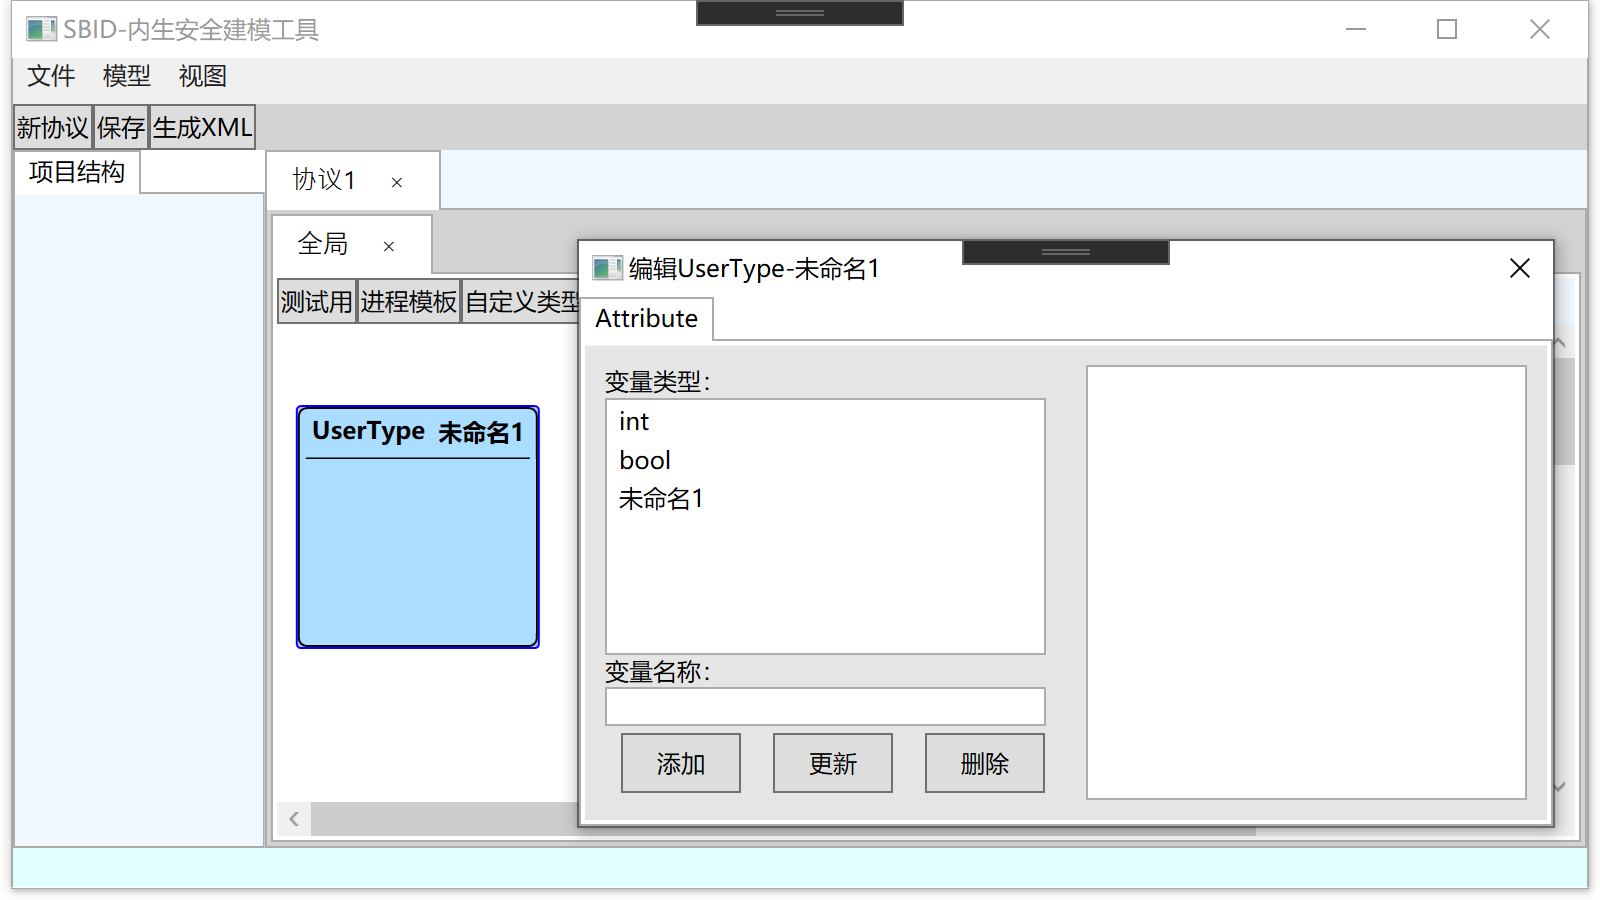
\includegraphics[width=12cm,height=6.75cm]{imgs/usertype_edit_window.png}
	\caption{自定义类型的编辑窗体}
	\label{usertype_edit_window}
\end{figure}
\par
每个自定义类型是以若干个类型为成员的新类型,在左侧选中已有类型,写入字段名称,点击添加按钮即可添加成员变量,如图\ref{usertype_edit_add}所示。
    \begin{figure}[h]
	\centering
	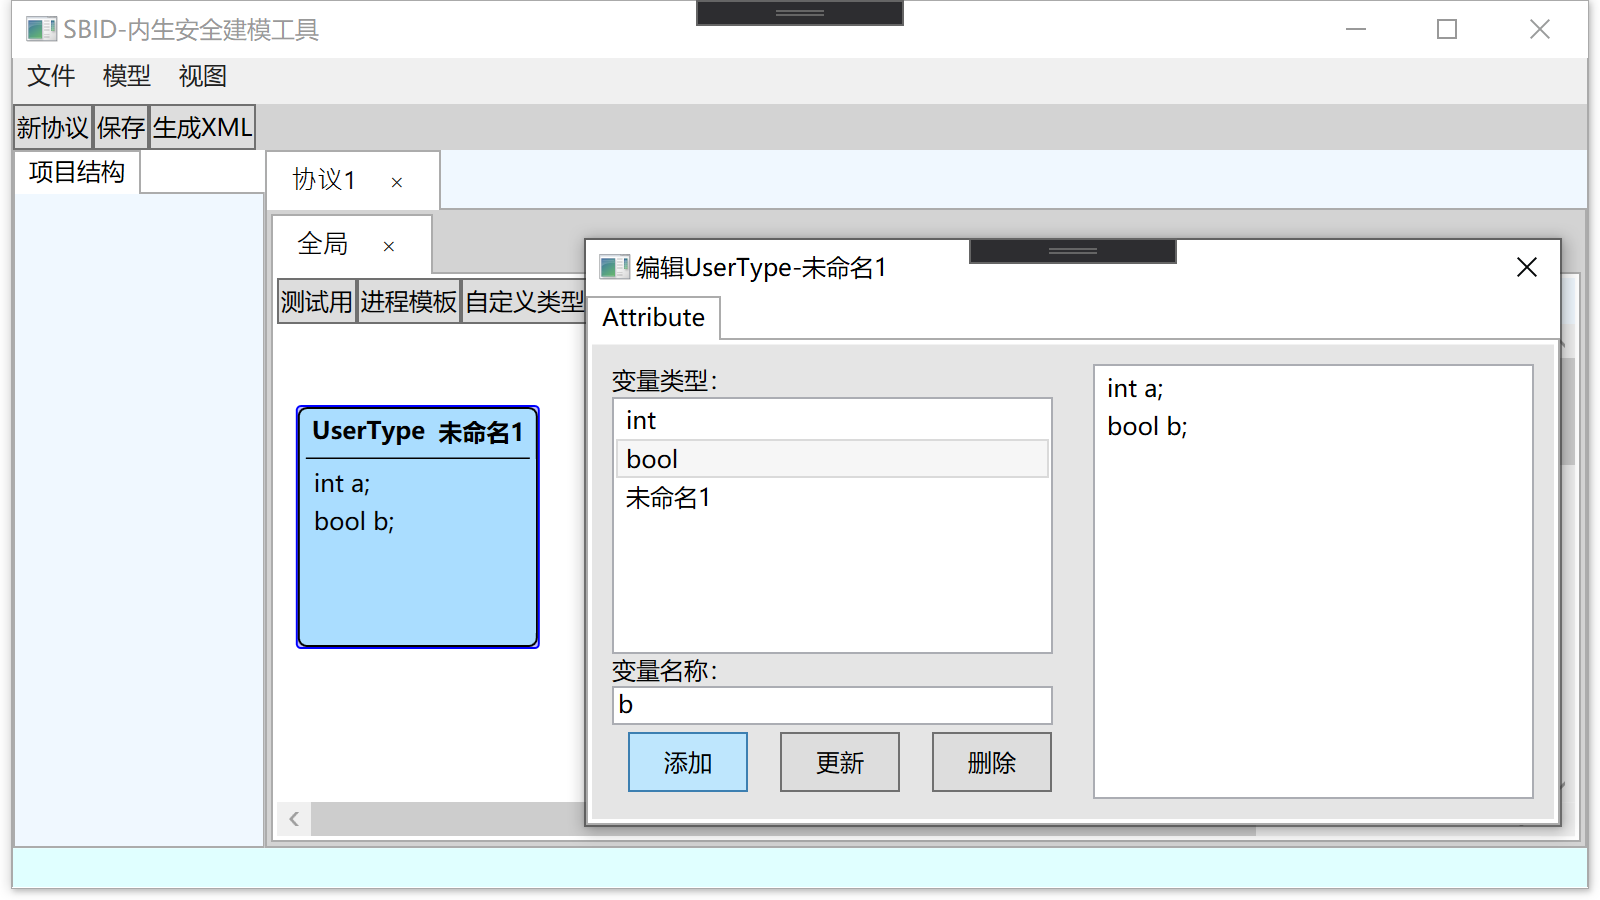
\includegraphics[width=12cm,height=6.75cm]{imgs/usertype_edit_add.png}
	\caption{添加成员变量}
	\label{usertype_edit_add}
	\end{figure}
\par
同理,选中右侧已存在的成员变量,可对其进行修改和删除。
\par
自定义类型可用在进程模板的属性、方法和通信方法的定义上。

\section{进程模板的Attribute}
在[协议>概览]下,点击小工具栏上的[进程模板]按钮,即可创建新的进程模板的类图,如图\ref{create_process}所示。
	\begin{figure}[h]
	\centering
	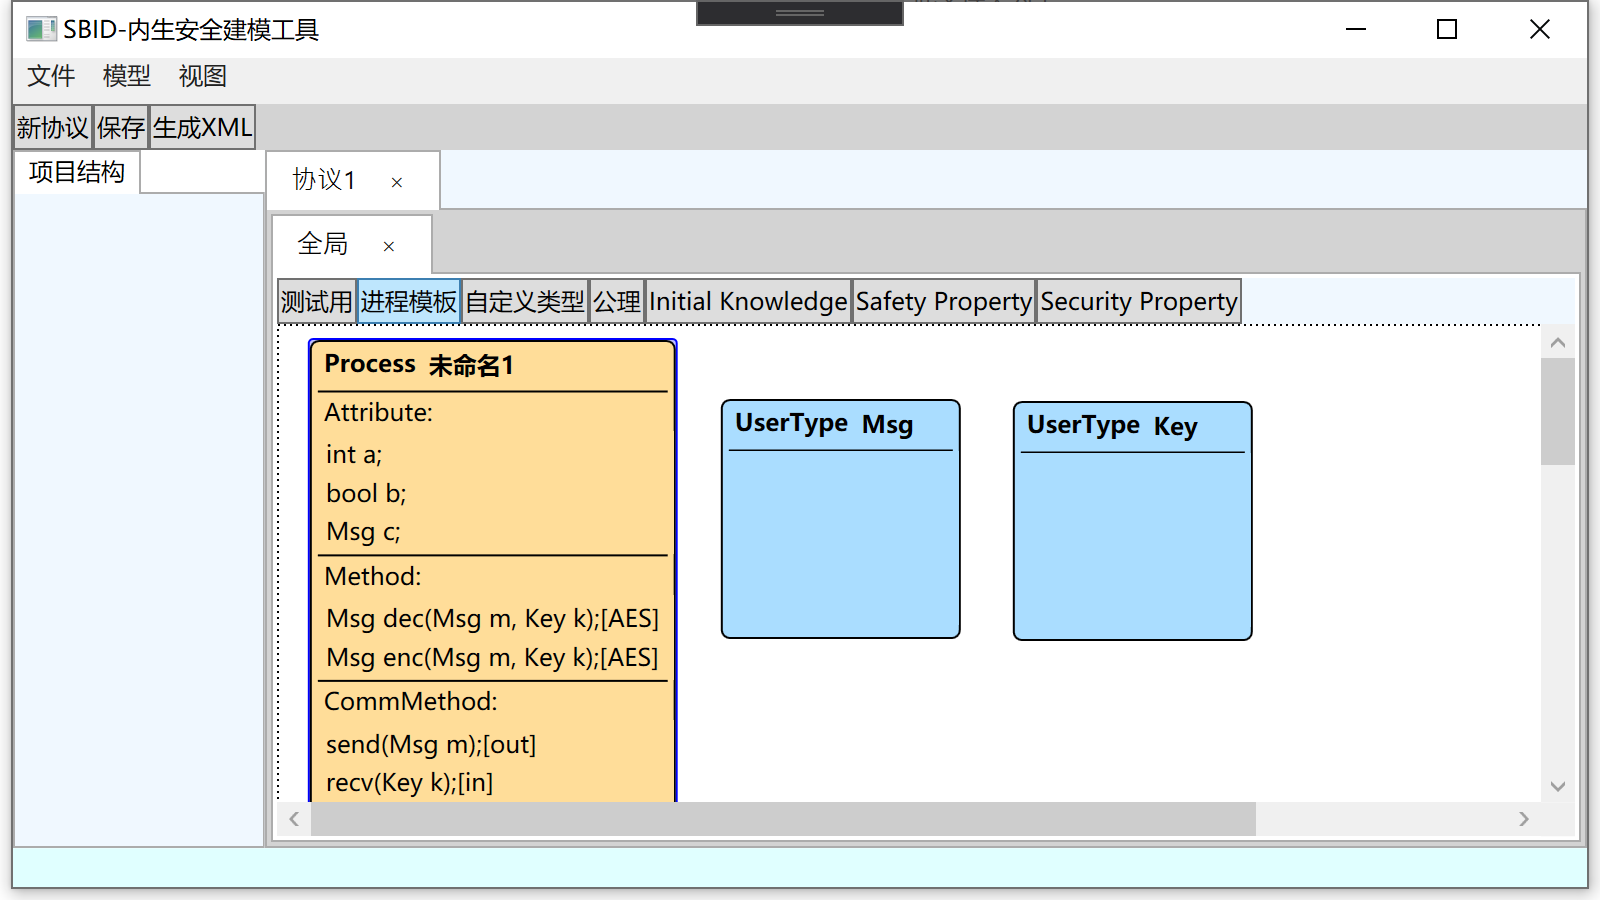
\includegraphics[width=12cm,height=6.75cm]{imgs/create_process.png}
	\caption{新创建的进程模板}
	\label{create_process}
	\end{figure}
\par
在进程模板的类图上右键,呼出右键菜单,点击[编辑Process],即可打开进程模板的编辑窗体。默认处在Attribute的编辑栏下,可对进程模板中的Attribute进行添加、修改和删除,如图\ref{process_edit_attribute}所示。
    \begin{figure}[h]
	\centering
	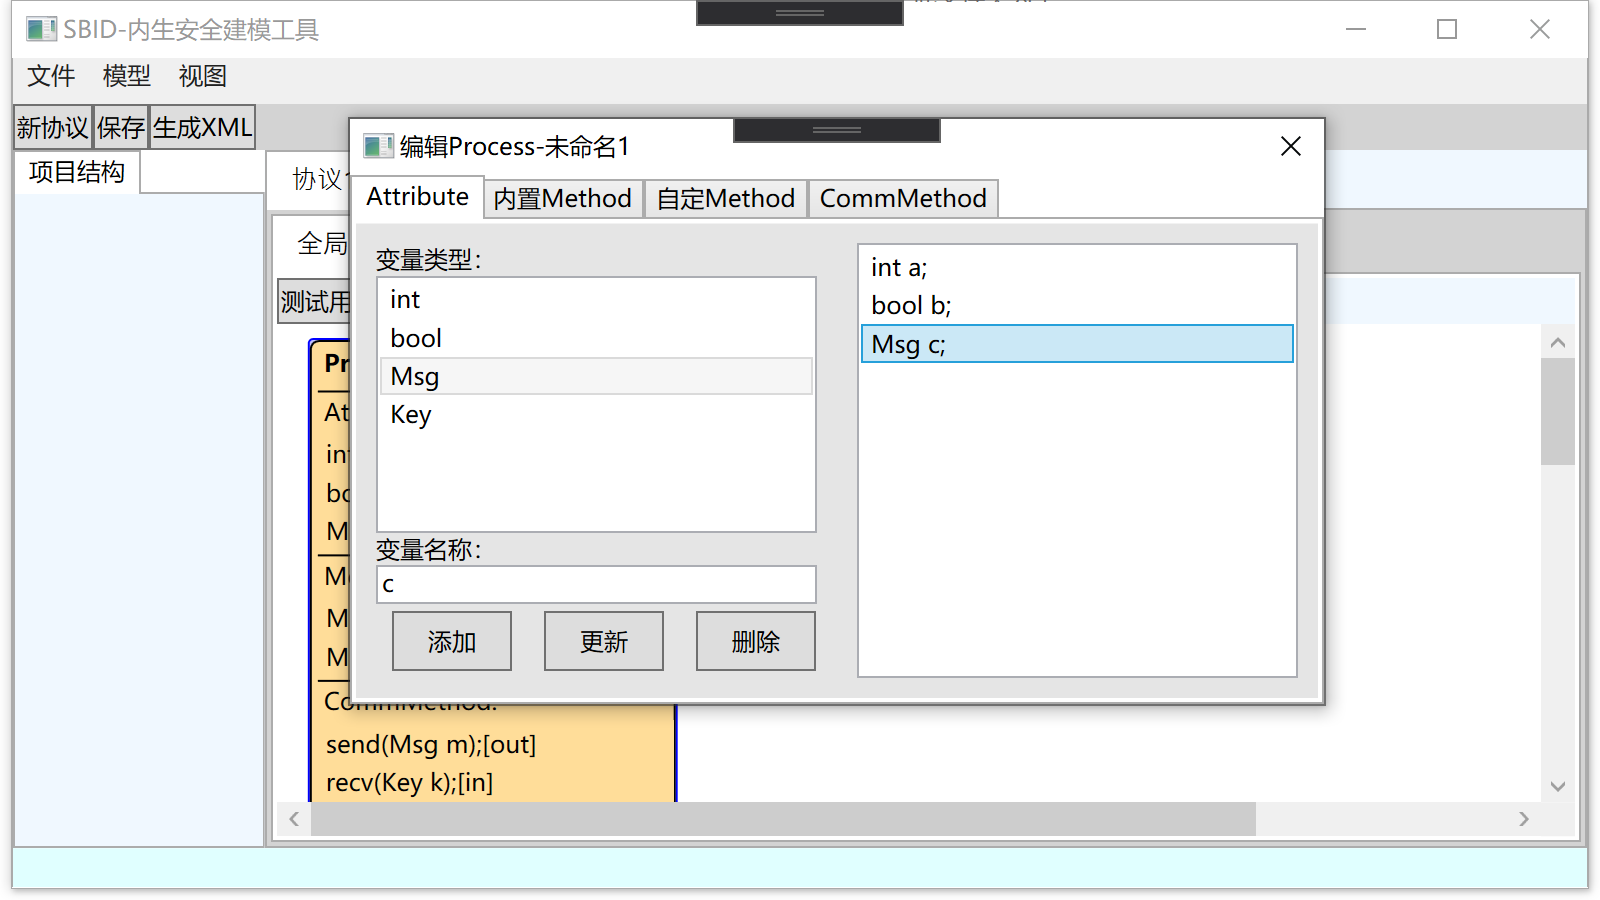
\includegraphics[width=12cm,height=6.75cm]{imgs/process_edit_attribute.png}
	\caption{编辑进程模板的Attribute}
	\label{process_edit_attribute}
	\end{figure}
\par
用户在协议中添加的自定义类型将和两种内置类型一起作为可添加的Attribute的类型。

\section{进程模板的Method}
同样地,在进程模板的编辑窗口可对其中组织的方法进行编辑。
\subsection{内置Method}
打开进程模板的编辑窗口,选择[内置Method]选项卡,可添加内置的Method,或将已有的函数修改为内置的Method,或删除已有的Method,如图\ref{process_edit_innermethod}所示。
    \begin{figure}[h]
	\centering
	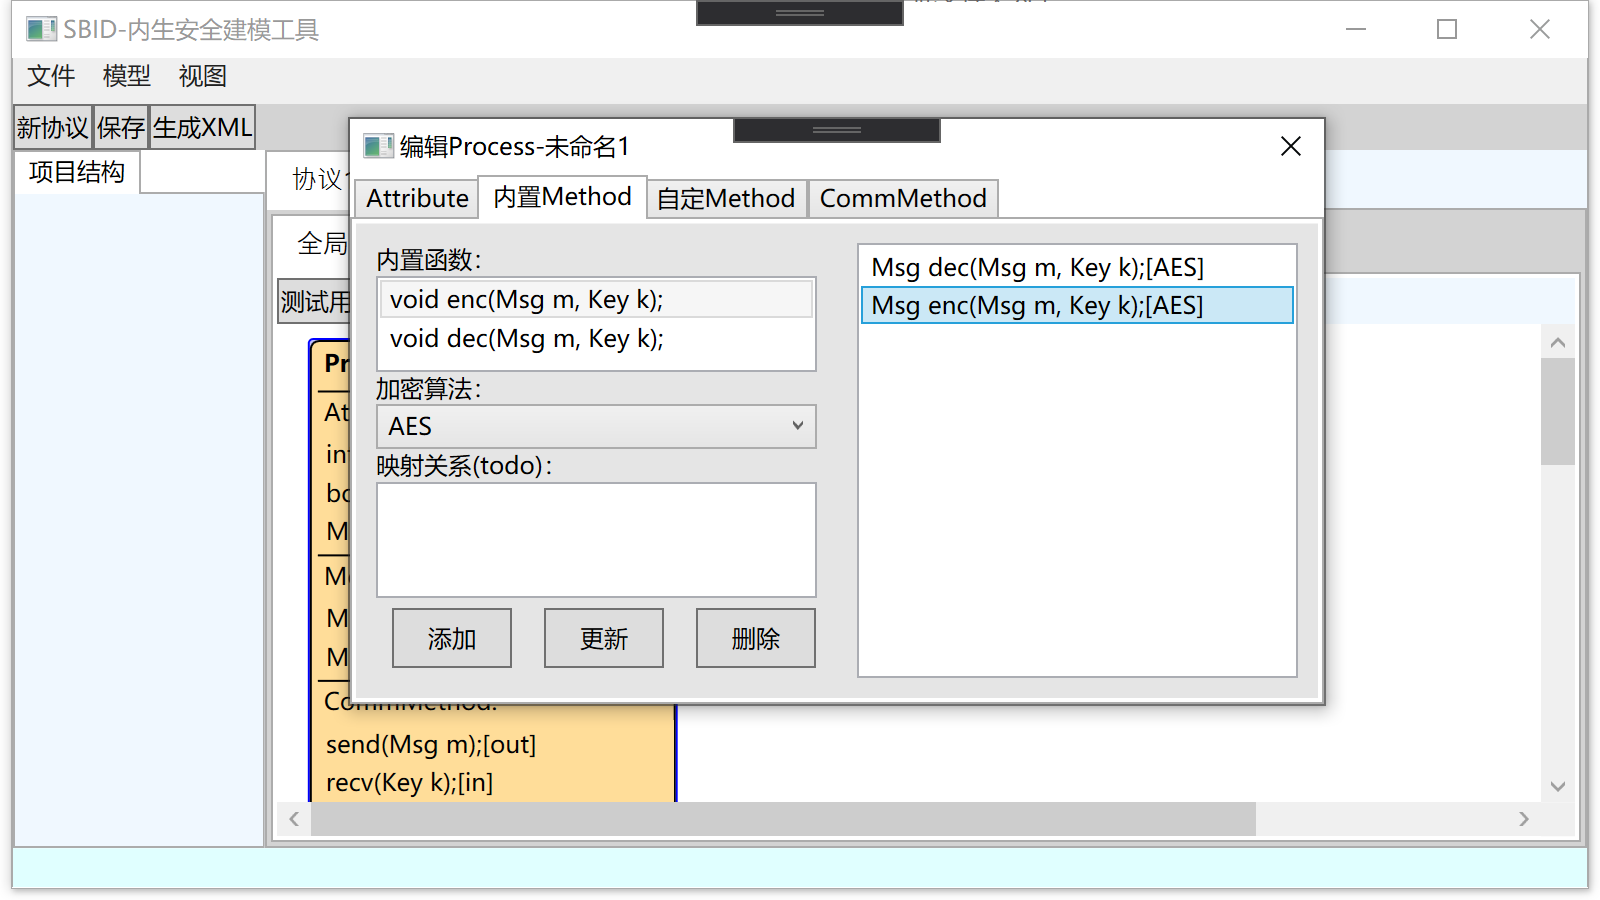
\includegraphics[width=12cm,height=6.75cm]{imgs/process_edit_innermethod.png}
	\caption{编辑进程模板的内置Method}
	\label{process_edit_innermethod}
	\end{figure}
\par
sbid内置了若干具有特定意义的Method,并需要与内置的加密算法组合,为进程模板所用。
\subsection{自定Method}
内置Method的功能未必能满足算法需求。打开进程模板的编辑窗口,选择[自定Method]选项卡,可以自行定制需要的Method,如图\ref{process_edit_zdmethod}所示。
\begin{figure}[h]
	\centering
	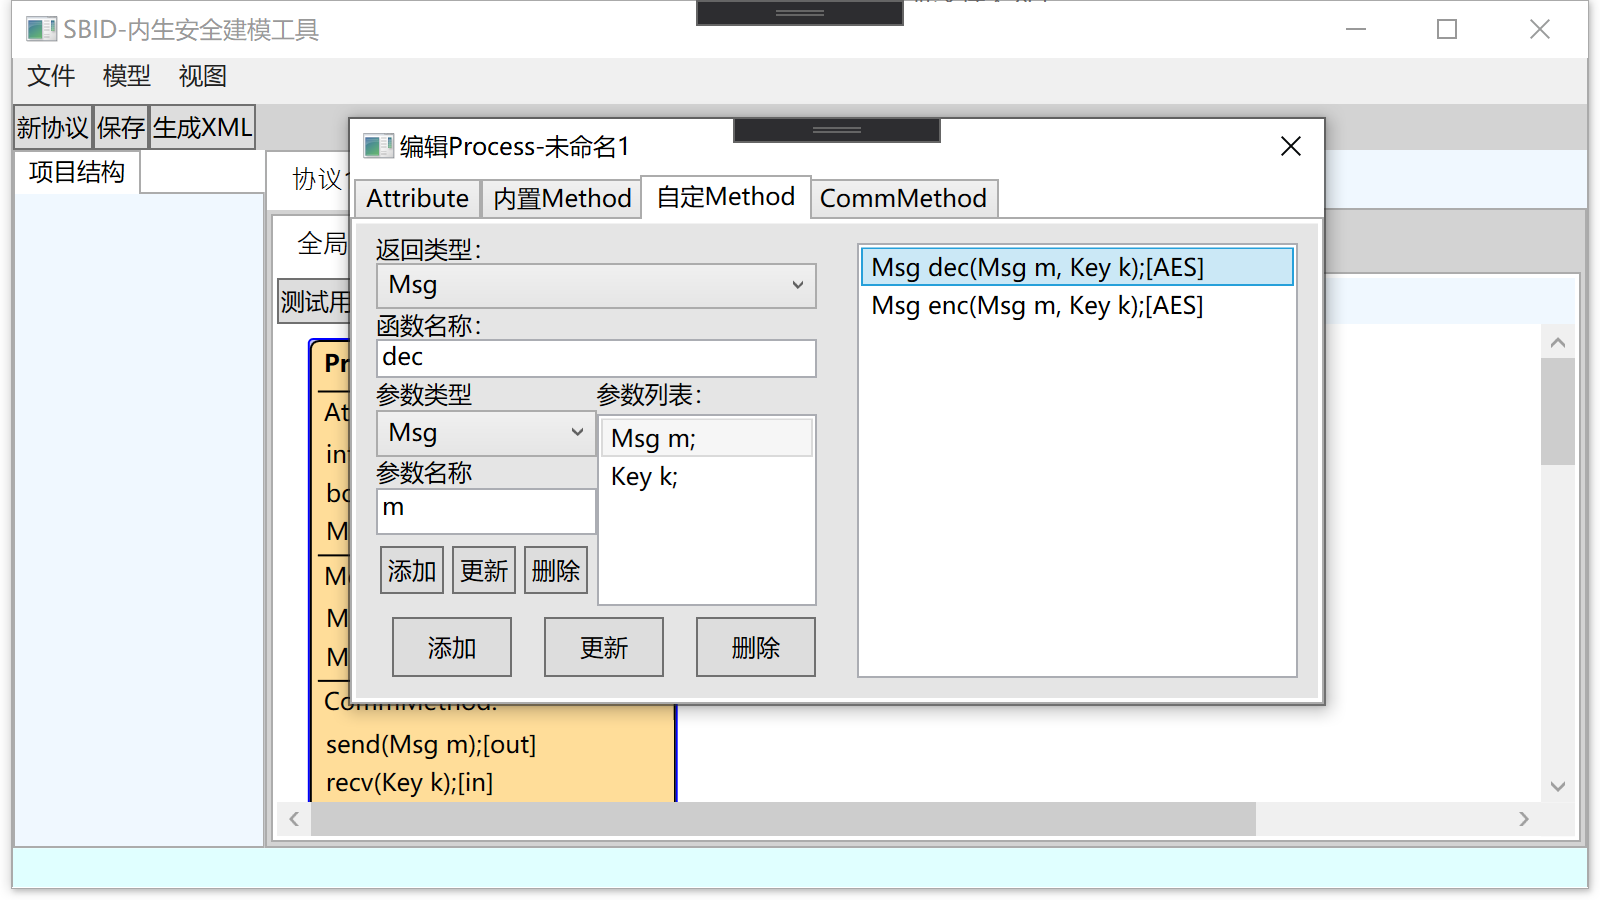
\includegraphics[width=12cm,height=6.75cm]{imgs/process_edit_zdmethod.png}
	\caption{编辑进程模板的自定Method}
	\label{process_edit_zdmethod}
	\end{figure}
\par
在自定Method的编辑选项卡中,左下角的区域用于向Method手动添加形参表。必须为Method指定返回值类型、方法名和形参表,才能成功添加或修改Method。

\section{进程模板的CommMethod}
进程模板的CommMethod用于定义进程模板之间的通信桥梁,和普通Method相比,CommMethod无需返回值,但需要有$in$和$out$指示是输入还是输出。CommMethod应当成对出现。
\par
打开进程模板的编辑窗口,选择[CommMethod]选项卡,可对CommMethod进行添加、修改和删除,如图\ref{process_edit_commmethod}所示。
\begin{figure}[h]
	\centering
	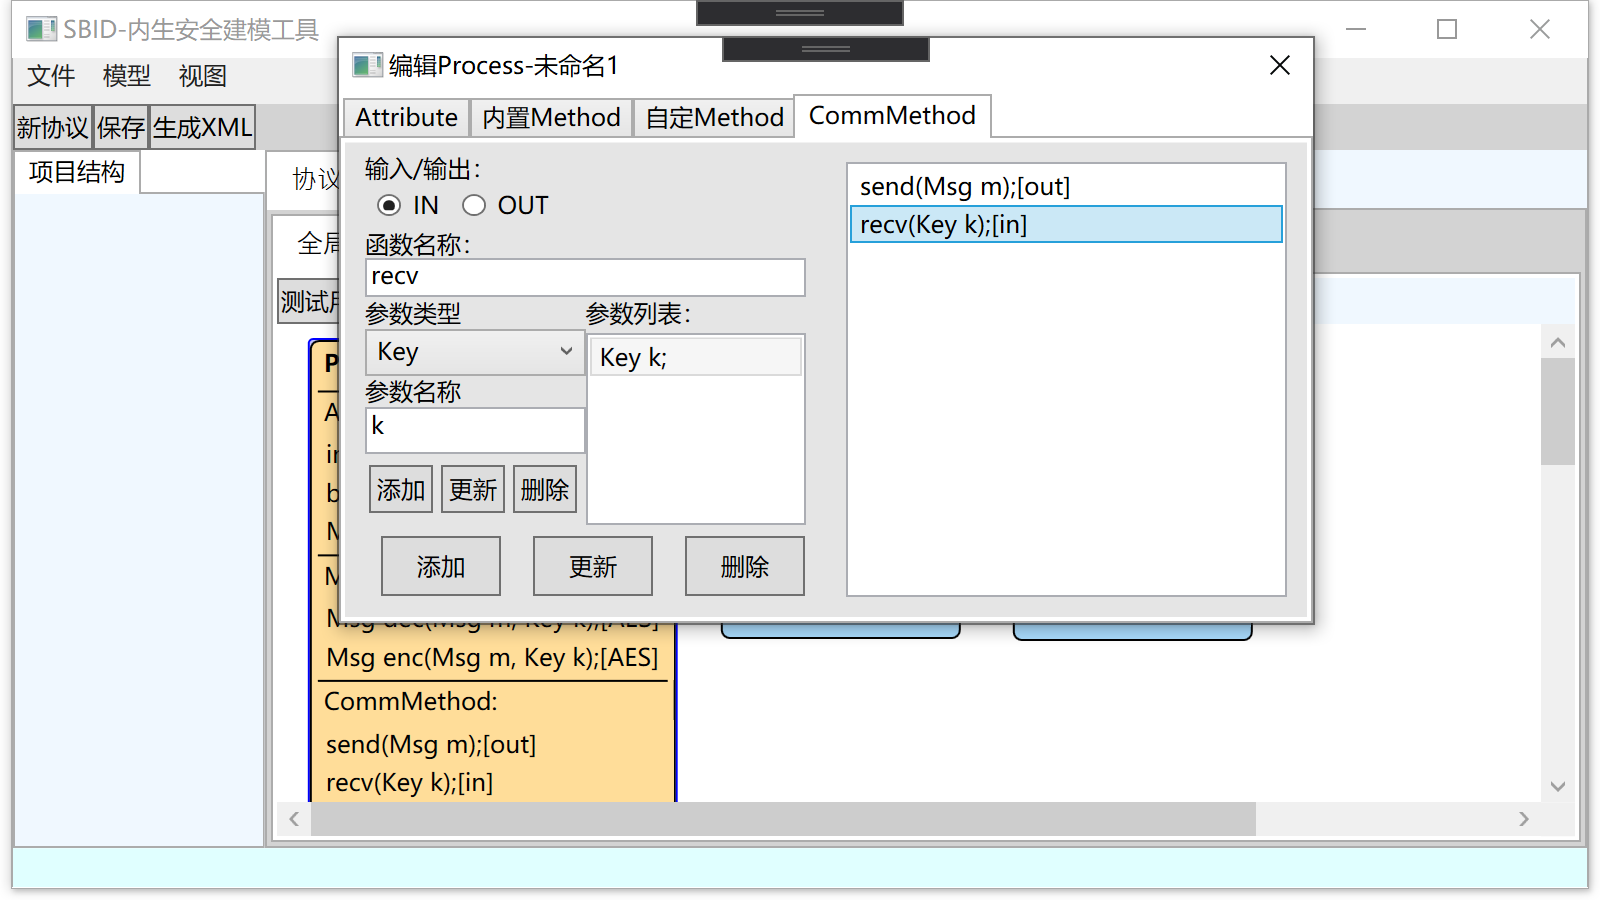
\includegraphics[width=12cm,height=6.75cm]{imgs/process_edit_commmethod.png}
	\caption{编辑进程模板的CommMethod}
	\label{process_edit_commmethod}
	\end{figure}
\par